%-------------------------------------------------------------------------------
\section{Findings}
%-------------------------------------------------------------------------------

Due to the time and resources available for our experiment, our efforts were limited 
to four targets, \texttt{exiv2}, \texttt{infotocap}, \texttt{mp3gain}, and 
\texttt{tcpdump}\textbf{(RQ2)}. Each of these were included in Fu et al.\cite{fu_autofz_2023} 
and are included in UNIFUZZ's\cite{li_unifuzz_2021} set of real-world programs for 
benchmarking fuzzers. As a baseline, UNIFUZZ's published counts of unique bugs are 
shown in figure \ref{fig:unifuzz_selections}.

\begin{figure}[ht!]
    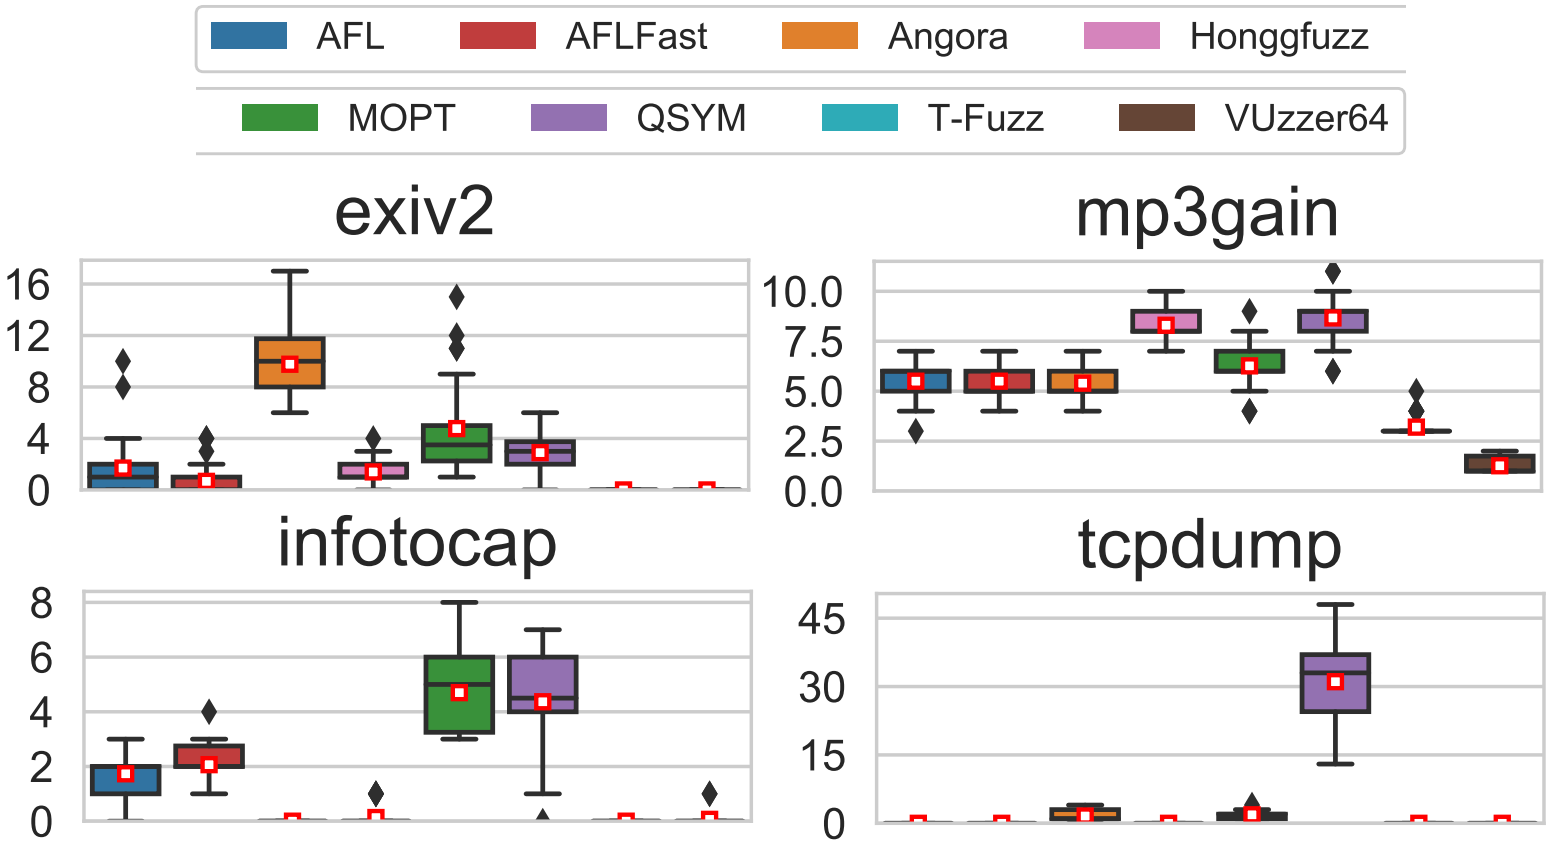
\includegraphics[width=0.5\textwidth]{figs/unifuzz_selections.png}
    \centering
    \caption{Counts of unique bugs found by the listed fuzzers, as documented in 
    UNIFUZZ\cite{li_unifuzz_2021}. These counts form the comparative baseline for 
    our work against Fu et al.\cite{fu_autofz_2023} and others.}
    \label{fig:unifuzz_selections}
\end{figure}

\subsection{Autofz on AMD64}

To confirm some of Fu et al.'s \cite{fu_autofz_2023} findings and validate our 
own \texttt{autofz} kits. Running on our AMD64 host, we were able to find the following
average counts of unique bugs, as shown in table \ref{amd64-benchmark-comparison}. 

As we can see, our average of unique bugs found in \texttt{infotocap} was consistent 
with Fu et al.\cite{fu_autofz_2023} and UNIFUZZ\cite{li_unifuzz_2021}. Their finding 
was based on ten (24 hour) fuzzing runs, ours was based on eight. While Fu et al. did 
not include metrics for the \texttt{mp3gain} target, our average was found by seven  
fuzzing runs and was consistent with the UNIFUZZ benchmark. Similarly, our average 
of 10 unique bugs was documented through only two fuzzing runs, but was consistent 
with UNIFUZZ and relatively close to Fu et al.'s finding.

The \texttt{tcpdump} target is an outlier in this set, but we note that only QSYM found 
a significant number of unique bugs, based on UNIFUZZ. 

\begin{table}[ht!]
    \begin{tabular}{llll}
        \toprule
         & amd64 & autofz\cite{fu_autofz_2023} & UNIFUZZ\cite{li_unifuzz_2021} \\
        \midrule
        infotocap & 4.09 & 5.50 & ~5 \\
        mp3gain & 8.38 & n/a & ~8 \\
        tcpdump & 0.15 & 1.9 &  ~30 \\
        exiv2 & 10.67 & 13.1 & ~10 \\
        \bottomrule
    \end{tabular}
    \caption{Comparison of average unique bugs found between our AMD64 host, original
    \texttt{autofz} and UNIFUZZ benchmarks.}
    \label{amd64-benchmark-comparison}
\end{table}

Figure \ref{fig:exiv2_compare_orig_amd64} displays bitmap density covered by the individual 
algorithms in our AMD64 implementation, as compared to a similar plot from Fu et al.
\cite{fu_autofz_2023}. While our recreation of autofz achieved lower bitmap coverage than 
the version published by Fu et al., our individual fuzzers also achieved lower bitmap 
coverage. As a result, our replica still outperformed all other individual fuzzers tested 
in our environment. We note this as our average number of unique bugs found in \texttt{exiv2} 
were similar to those found by Fu et al. 

Likewise, we compare bitmap coverage of \texttt{tcpdump} on our AMD64 host to the findings 
in the original \texttt{autofz} report\cite{fu_autofz_2023}, shown in figure 
\ref{fig:tcpdump_compare_orig_amd64}.

\begin{figure}[ht!]
    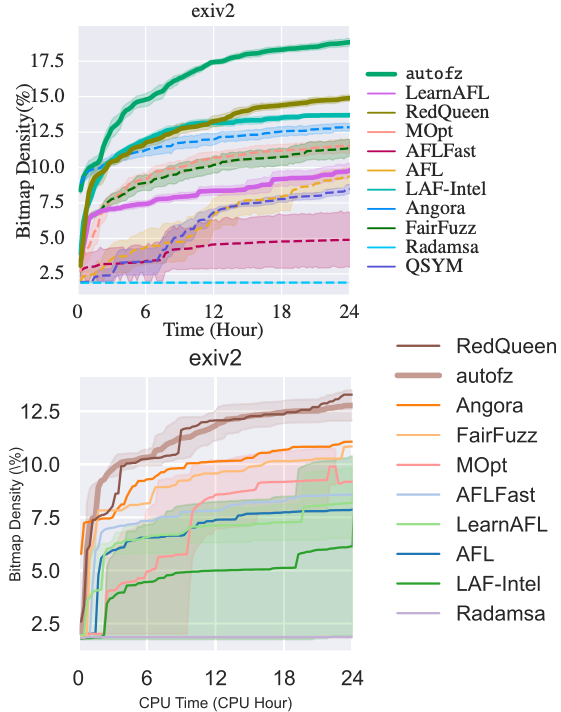
\includegraphics[width=0.5\textwidth]{figs/exiv2_compare_orig_amd64.png}
    \centering
    \caption{A comparison of bitmap density covered in the original\cite{fu_autofz_2023} (shown 
    on top) and our coverage (shown on bottom) during initial fuzzing of \texttt{exiv2}.}
    \label{fig:exiv2_compare_orig_amd64}
\end{figure}

\begin{figure}[ht!]
    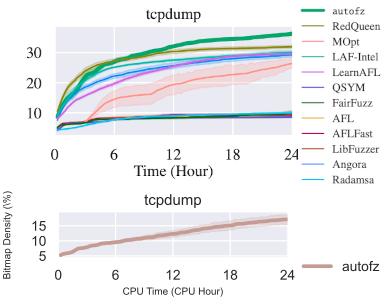
\includegraphics[width=0.5\textwidth]{figs/tcpdump_compare_orig_amd64.png}
    \centering
    \caption{A comparison of bitmap density covered in the original\cite{fu_autofz_2023} (shown 
    on top) and our coverage (shown on bottom) during initial fuzzing of \texttt{tcpdump}.}
    \label{fig:tcpdump_compare_orig_amd64}
\end{figure}

\subsection{Autofz on ARM64}

Testing also shows that the ARM64 compatible \texttt{autofz} performs similarly to the unmodified 
AMD64 \texttt{autofz}. Table \ref{arm64-benchmark-comparison} provides a side-by-side comparison 
of the average numbers of unique bugs found with our ARM64 kit, AMD64 host, the original 
\texttt{autofz} paper, and the UNIFUZZ benchmark.

We consistently found many more bugs in \texttt{exiv2} on ARM64, over the course of ten fuzzing 
runs. At this time, we recommend further study to validate these bugs and understand why this 
behavior was observed. 

Bitmap density coverage of AMD64 \texttt{autofz} is plotted alogside our ARM64 \texttt{autofz} in figure 
\ref{fig:tcpdump_compare_orig_arm64}. After 24 hours, both implementations achieved similar bitmap coverage.
AMD64 \texttt{Autofz}'s bitmap coverage grew linearly while ARM64 \texttt{autofz} followed a 
logarithmic trend. Consequently, the AMD64 \texttt{autofz} took longer to achieve the same bitmap coverage. 

\begin{table}[ht!]
    \begin{tabular}{lllll}
        \toprule
         & arm64 & amd64 & autofz & UNIFUZZ \\
        \midrule
        infotocap & 4.77 & 4.09 & 5.50 & ~5 \\
        mp3gain & 8.00 & 8.67 & n/a & ~8 \\
        tcpdump & 0.38 & 0.15 & 1.9 &  ~30 \\
        exiv2 & 33.50 & 10.00 & 13.1 & ~10 \\
        \bottomrule
        \end{tabular}
        \caption{Comparison of average unique bugs found between ARMy Fuzzing (ARM64), our AMD64 
        host, original \texttt{autofz} and UNIFUZZ benchmarks.}
        \label{arm64-benchmark-comparison}
    \end{table}

\begin{figure}
    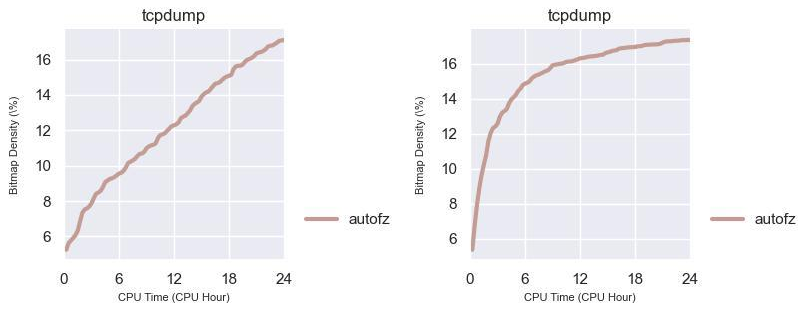
\includegraphics[width=0.52\textwidth]{figs/tcpdump_compare_orig_arm64.png}
    \centering
    \caption{A comparison of bitmap density covered in AMD64 \texttt{autofz} and our ARM64 implementation
    coverage during fuzzing of tcpdump}
    \label{fig:tcpdump_compare_orig_arm64}
\end{figure}

Bug coverage of our ARM64 fuzzing campaign against tcpdump is plotted in figure \ref{figs:tcp_compare_orig_arm64_ub.png}, 
shown as a comparison are results from Fu et al.\cite{fu_autofz_2023}. While the ARM64 adaptation of 
\texttt{autofz} achieved similar performance to the original in bitmap coverage, it outperformed the 
original in bug discovery. Since the other targets followed similar trends when fuzzed with ARM64 
\texttt{autofz}, \texttt{autofz} can be successfully adapted for the ARM64 architecture.

\begin{figure}
    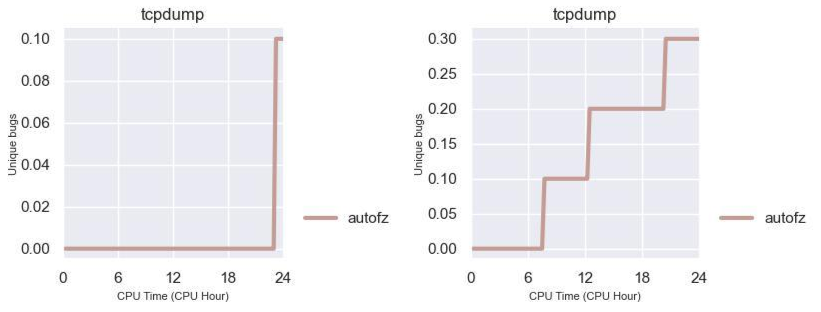
\includegraphics[width=0.52\textwidth]{figs/tcpdump_compare_orig_arm64_ub.png}
    \centering
    \caption{A comparison of bug discovery in AMD64 \texttt{autofz} and our ARM64 implementation
    coverage during fuzzing of tcpdump}
    \label{figs:tcp_compare_orig_arm64_ub.png}
\end{figure}

\subsection{Additional Metrics for Autofz}

The outcomes of the new resource allocation algorithms on tcpdump in ARM64 and AMD64 are documented in 
\ref{figs:tcpdump_algo_compare.png}. The outcomes of these algorithms were not consistent. While the 
ub-bitmap algorithm outperforms the others when tested on the AMD64, a consistent winner does not 
present when the algorithms are tested in the ARM64 environment.


In table \ref{arm64-additional-metrics}, we document the average number of bugs found by each of 
our fuzzing algorithms on ARM64, including our three new algorithms that consider unique bugs as a 
discrimination metric. In all of these cases, the \texttt{bitmap} algorithm is equivalent to autofz running without 
specifying a discriminator (i.e. default). Due to time constraints, we did not complete 

\begin{table}
    \begin{tabular}{lllll}
        \toprule
         & ub & ub-bitmap & bitmap-ub & bitmap \\
        \midrule
        infotocap & 4.00 & 3.00 & 1.00 & 4.77 \\
        mp3gain & 7.40 & 8.83 & 8.0 & 8.0 \\       
        tcpdump & 0.00 & 0.00 & 0.00 & 0.38 \\
        exiv2 & 34.0 & 44.0 & 27.0 & 29.80 \\
        \bottomrule
    \end{tabular}
    \caption{Comparison of average unique bugs found between ARMy Fuzzing (ARM64), our AMD64 
    host, original \texttt{autofz} and UNIFUZZ benchmarks.}
    \label{arm64-additional-metrics}
\end{table}

\begin{figure}
    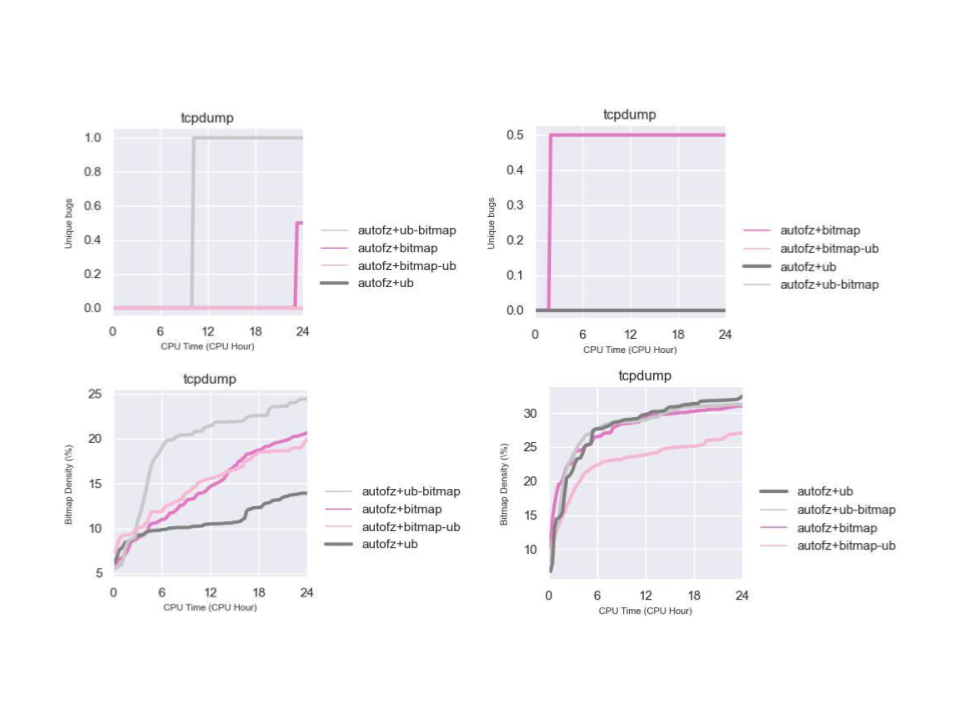
\includegraphics[width=0.52\textwidth]{figs/tcpdump_algo_compare.png}
    \centering
    \caption{The outcomes of the new resource allocation algorithms on tcpdump when executed on the AMD64 and ARM64 architectures}
    \label{figs:tcpdump_algo_compare.png}
\end{figure}

The inverse of this pattern can be identifed when the new resource allocation algorithms are executed on infotocap in 
\ref{figs:infotocap_algo_compare.png}. When the new algorithms are tested on infotocap in AMD64 \texttt{autofz}, one does not achieve better
bitmap coverage and bug discovery, but when the new algorithms are tested on ARM64 \texttt{autofz}, ub-bitmap is the best algorithm.

\begin{figure}

    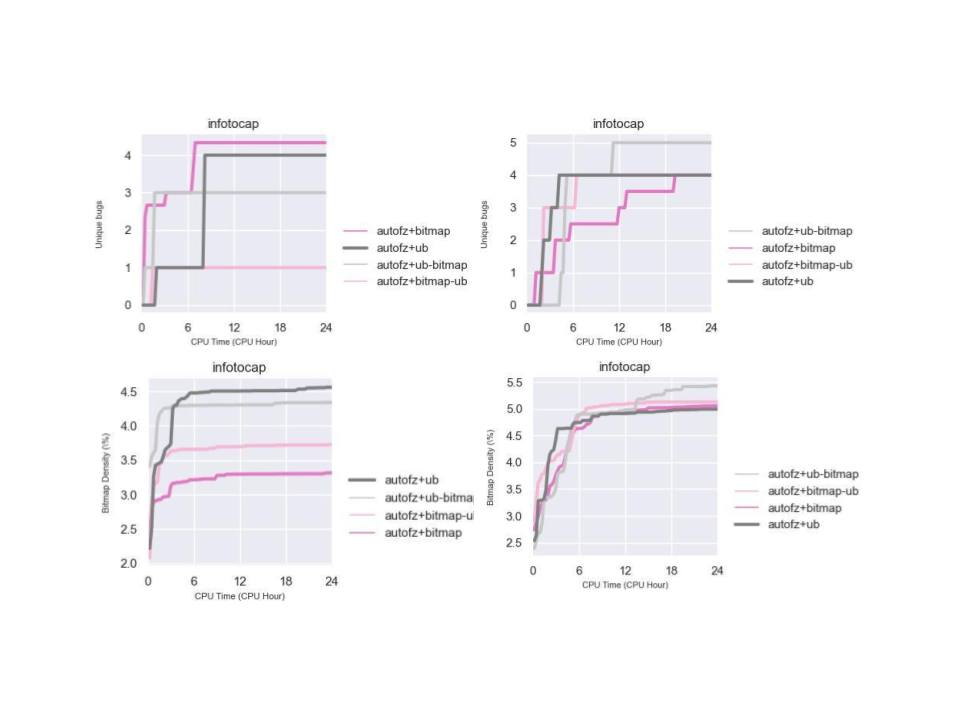
\includegraphics[width=0.52\textwidth]{figs/infotocap_algo_compare.png}
    \centering
    \caption{The outcomes of the new resource allocation algorithms on infotocap when executed on the AMD64 and ARM64 architectures}
    \label{figs:infotocap_algo_compare.png}
\end{figure}

As a result of these inconsistencies, one algorithm cannot be identifed as better than the others at this time.


